\documentclass[tikz,border=2pt]{standalone}
\usepackage[T1]{fontenc}
\usepackage{helvet}
\renewcommand{\familydefault}{\sfdefault}
\usepackage{amsmath}
\usetikzlibrary{arrows.meta,positioning,calc,fit,backgrounds}

\definecolor{cAgent}{HTML}{DCE9F5}
\definecolor{cAgentB}{HTML}{6C8EBF}
\definecolor{cProp}{HTML}{FBE5D0}
\definecolor{cPropB}{HTML}{D79B5B}
\definecolor{cEval}{HTML}{DFF0E4}
\definecolor{cEvalB}{HTML}{5B9A6E}
\definecolor{cCert}{HTML}{ECE7F5}
\definecolor{cCertB}{HTML}{8A6FB5}
\definecolor{cGrey}{HTML}{555F6B}
\definecolor{cWall}{HTML}{B03A2E}

\begin{document}
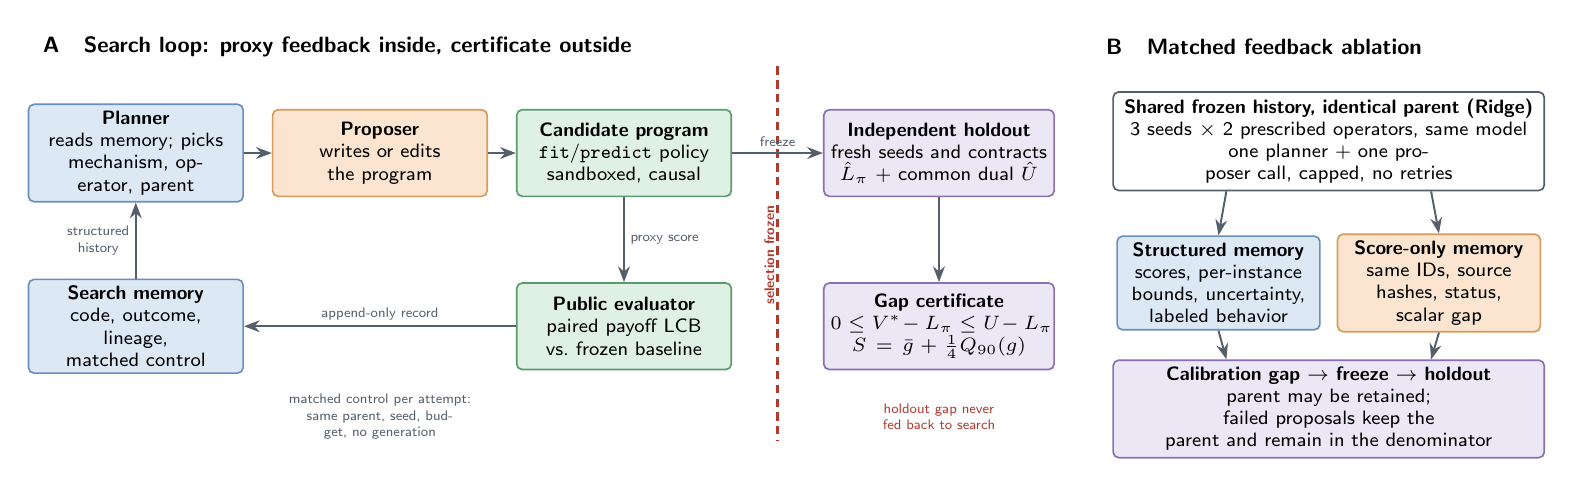
\begin{tikzpicture}[
  font=\scriptsize,
  >={Stealth[length=2mm,width=1.5mm]},
  box/.style={draw, rounded corners=2pt, line width=0.6pt, align=center,
              inner sep=2.5pt, minimum height=11mm, text width=2.55cm},
  agent/.style={box, fill=cAgent, draw=cAgentB},
  prop/.style={box, fill=cProp, draw=cPropB},
  eval/.style={box, fill=cEval, draw=cEvalB},
  cert/.style={box, fill=cCert, draw=cCertB},
  arr/.style={->, line width=0.7pt, color=cGrey},
  lab/.style={font=\tiny, color=cGrey, align=center, inner sep=1pt},
  panel/.style={font=\footnotesize\bfseries, anchor=west}
]

%%%%%%%%%%%%%%%%%%%%%%%%%%%%%%%%%%%%%%%%%%%%%%%%%%%%%%%%%%%%%%%%%%%%%%%%
% Panel A
%%%%%%%%%%%%%%%%%%%%%%%%%%%%%%%%%%%%%%%%%%%%%%%%%%%%%%%%%%%%%%%%%%%%%%%%
\node[panel] at (-1.3,3.55) {A\quad Search loop: proxy feedback inside, certificate outside};

\node[agent] (ctx)  at (0,2.2)   {\textbf{Planner}\\reads memory; picks\\mechanism, operator, parent};
\node[prop]  (prop) at (3.1,2.2) {\textbf{Proposer}\\writes or edits\\the program};
\node[eval]  (cand) at (6.2,2.2) {\textbf{Candidate program}\\\texttt{fit}/\texttt{predict} policy\\sandboxed, causal};
\node[eval]  (pub)  at (6.2,0)   {\textbf{Public evaluator}\\paired payoff LCB\\vs.\ frozen baseline};
\node[agent] (eb)   at (0,0)     {\textbf{Search memory}\\code, outcome,\\lineage, matched control};

\draw[arr] (ctx) -- (prop);
\draw[arr] (prop) -- (cand);
\draw[arr] (cand) -- node[lab, right=1pt] {proxy score} (pub);
\draw[arr] (pub) -- node[lab, above=1pt] {append-only record} (eb);
\draw[arr] (eb) -- node[lab, left=1pt] {structured\\history} (ctx);
\node[lab, text width=3.2cm] at (3.1,-1.15)
  {matched control per attempt:\\same parent, seed, budget, no generation};

% wall
\draw[line width=1.1pt, dash pattern=on 3pt off 2pt, color=cWall] (8.15,3.3) -- (8.15,-1.45);
\node[font=\tiny\bfseries, color=cWall, rotate=90, anchor=south, inner sep=1pt] at (8.15,0.9) {selection frozen};

\node[cert, text width=2.75cm] (hold) at (10.2,2.2) {\textbf{Independent holdout}\\fresh seeds and contracts\\$\hat L_\pi$ + common dual $\hat U$};
\node[cert, text width=2.75cm] (gap)  at (10.2,0)   {\textbf{Gap certificate}\\${0\le V^*\!-L_\pi\le U\!-L_\pi}$\\$S=\bar g+\tfrac14 Q_{90}(g)$};
\draw[arr] (cand) -- node[lab, above=1pt] {freeze} (hold);
\draw[arr] (hold) -- (gap);
\node[lab, color=cWall, text width=2.4cm] at (10.2,-1.15) {holdout gap never\\fed back to search};

%%%%%%%%%%%%%%%%%%%%%%%%%%%%%%%%%%%%%%%%%%%%%%%%%%%%%%%%%%%%%%%%%%%%%%%%
% Panel B
%%%%%%%%%%%%%%%%%%%%%%%%%%%%%%%%%%%%%%%%%%%%%%%%%%%%%%%%%%%%%%%%%%%%%%%%
\node[panel] at (12.2,3.55) {B\quad Matched feedback ablation};

\node[box, fill=white, draw=cGrey, text width=5.3cm, minimum height=9mm] (shared) at (15.15,2.35)
  {\textbf{Shared frozen history, identical parent (Ridge)}\\3 seeds $\times$ 2 prescribed operators, same model\\one planner + one proposer call, capped, no retries};

\node[agent, text width=2.4cm] (sm) at (13.75,0.55)
  {\textbf{Structured memory}\\scores, per-instance\\bounds, uncertainty,\\labeled behavior};
\node[prop, text width=2.4cm] (so) at (16.55,0.55)
  {\textbf{Score-only memory}\\same IDs, source\\hashes, status,\\scalar gap};

\draw[arr] ($(shared.south)+(-1.3,0)$) -- (sm.north);
\draw[arr] ($(shared.south)+(1.3,0)$) -- (so.north);

\node[cert, text width=5.3cm, minimum height=9mm] (sel) at (15.15,-1.05)
  {\textbf{Calibration gap $\rightarrow$ freeze $\rightarrow$ holdout}\\parent may be retained; failed proposals keep the\\parent and remain in the denominator};
\draw[arr] (sm.south) -- ($(sel.north)+(-1.3,0)$);
\draw[arr] (so.south) -- ($(sel.north)+(1.3,0)$);

\end{tikzpicture}
\end{document}
